%% LyX 2.0.5.1 created this file.  For more info, see http://www.lyx.org/.
%% Do not edit unless you really know what you are doing.
\documentclass{article}\usepackage{graphicx, color}
%% maxwidth is the original width if it is less than linewidth
%% otherwise use linewidth (to make sure the graphics do not exceed the margin)
\makeatletter
\def\maxwidth{ %
  \ifdim\Gin@nat@width>\linewidth
    \linewidth
  \else
    \Gin@nat@width
  \fi
}
\makeatother

\IfFileExists{upquote.sty}{\usepackage{upquote}}{}
\definecolor{fgcolor}{rgb}{0.2, 0.2, 0.2}
\newcommand{\hlnumber}[1]{\textcolor[rgb]{0,0,0}{#1}}%
\newcommand{\hlfunctioncall}[1]{\textcolor[rgb]{0.501960784313725,0,0.329411764705882}{\textbf{#1}}}%
\newcommand{\hlstring}[1]{\textcolor[rgb]{0.6,0.6,1}{#1}}%
\newcommand{\hlkeyword}[1]{\textcolor[rgb]{0,0,0}{\textbf{#1}}}%
\newcommand{\hlargument}[1]{\textcolor[rgb]{0.690196078431373,0.250980392156863,0.0196078431372549}{#1}}%
\newcommand{\hlcomment}[1]{\textcolor[rgb]{0.180392156862745,0.6,0.341176470588235}{#1}}%
\newcommand{\hlroxygencomment}[1]{\textcolor[rgb]{0.43921568627451,0.47843137254902,0.701960784313725}{#1}}%
\newcommand{\hlformalargs}[1]{\textcolor[rgb]{0.690196078431373,0.250980392156863,0.0196078431372549}{#1}}%
\newcommand{\hleqformalargs}[1]{\textcolor[rgb]{0.690196078431373,0.250980392156863,0.0196078431372549}{#1}}%
\newcommand{\hlassignement}[1]{\textcolor[rgb]{0,0,0}{\textbf{#1}}}%
\newcommand{\hlpackage}[1]{\textcolor[rgb]{0.588235294117647,0.709803921568627,0.145098039215686}{#1}}%
\newcommand{\hlslot}[1]{\textit{#1}}%
\newcommand{\hlsymbol}[1]{\textcolor[rgb]{0,0,0}{#1}}%
\newcommand{\hlprompt}[1]{\textcolor[rgb]{0.2,0.2,0.2}{#1}}%

\usepackage{framed}
\makeatletter
\newenvironment{kframe}{%
 \def\at@end@of@kframe{}%
 \ifinner\ifhmode%
  \def\at@end@of@kframe{\end{minipage}}%
  \begin{minipage}{\columnwidth}%
 \fi\fi%
 \def\FrameCommand##1{\hskip\@totalleftmargin \hskip-\fboxsep
 \colorbox{shadecolor}{##1}\hskip-\fboxsep
     % There is no \\@totalrightmargin, so:
     \hskip-\linewidth \hskip-\@totalleftmargin \hskip\columnwidth}%
 \MakeFramed {\advance\hsize-\width
   \@totalleftmargin\z@ \linewidth\hsize
   \@setminipage}}%
 {\par\unskip\endMakeFramed%
 \at@end@of@kframe}
\makeatother

\definecolor{shadecolor}{rgb}{.97, .97, .97}
\definecolor{messagecolor}{rgb}{0, 0, 0}
\definecolor{warningcolor}{rgb}{1, 0, 1}
\definecolor{errorcolor}{rgb}{1, 0, 0}
\newenvironment{knitrout}{}{} % an empty environment to be redefined in TeX

\usepackage{alltt}
\usepackage[sc]{mathpazo}
\usepackage{geometry}
\geometry{verbose,tmargin=2.5cm,bmargin=2.5cm,lmargin=2.5cm,rmargin=2.5cm}
\setcounter{secnumdepth}{2}
\setcounter{tocdepth}{2}
\usepackage{url}
\usepackage[unicode=true,pdfusetitle,
 bookmarks=true,bookmarksnumbered=true,bookmarksopen=true,bookmarksopenlevel=2,
 breaklinks=false,pdfborder={0 0 1},backref=false,colorlinks=false]
 {hyperref}
\hypersetup{
 pdfstartview={XYZ null null 1}}
\usepackage{breakurl}
\begin{document}





\title{Stat 2025 - HW 8}
\author{Michael Discenza}

\maketitle

\section*{Setting up data}

\begin{knitrout}
\definecolor{shadecolor}{rgb}{0.969, 0.969, 0.969}\color{fgcolor}\begin{kframe}
\begin{alltt}
SAH <- \hlfunctioncall{read.table}(\hlstring{"http://stat.columbia.edu/~madigan/W2025/data/SAHmissing.txt"}, 
    header = TRUE, sep = \hlstring{"\textbackslash{}t"})
SAH <- \hlfunctioncall{na.exclude}(SAH)  \hlcomment{# only use the records for which we have the response variable}
validation.cases <- \hlfunctioncall{sample}(1:\hlfunctioncall{dim}(SAH)[1], 42, replace = F)  \hlcomment{# randomly select 42 records to hold out}
validation.data <- SAH[validation.cases, ]
training.data <- SAH[-validation.cases, ]
\end{alltt}
\end{kframe}
\end{knitrout}


\section*{Fitting a Classification Tree Model}

First we fit a full single tree.  We look at the plot of cross validation errors against the various complexity parameters, which correspond to trees of different sizes
\begin{knitrout}
\definecolor{shadecolor}{rgb}{0.969, 0.969, 0.969}\color{fgcolor}\begin{kframe}
\begin{alltt}
\hlfunctioncall{library}(rpart)
tree1 <- \hlfunctioncall{rpart}(chd ~ ., data = training.data, method = \hlstring{"class"})
\hlfunctioncall{plotcp}(tree1)
\end{alltt}
\end{kframe}
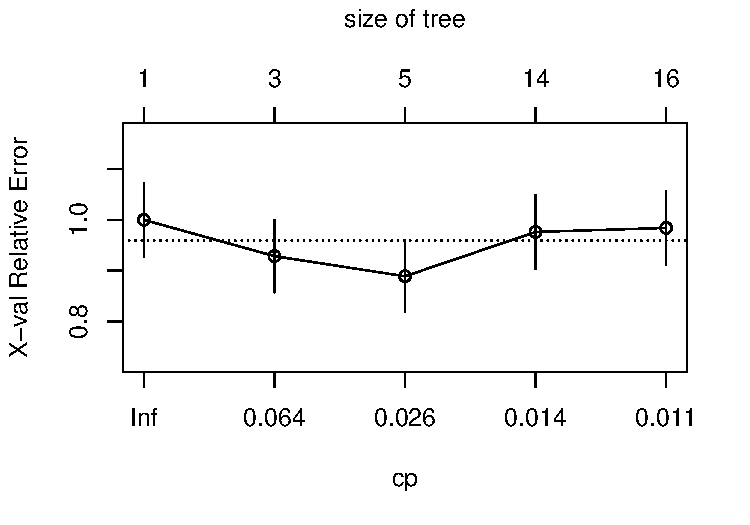
\includegraphics[width=\maxwidth]{figure/tree11} 
\begin{kframe}\begin{alltt}
\hlfunctioncall{plot}(tree1)
\hlfunctioncall{text}(tree1, cex = 0.7)
\end{alltt}
\end{kframe}
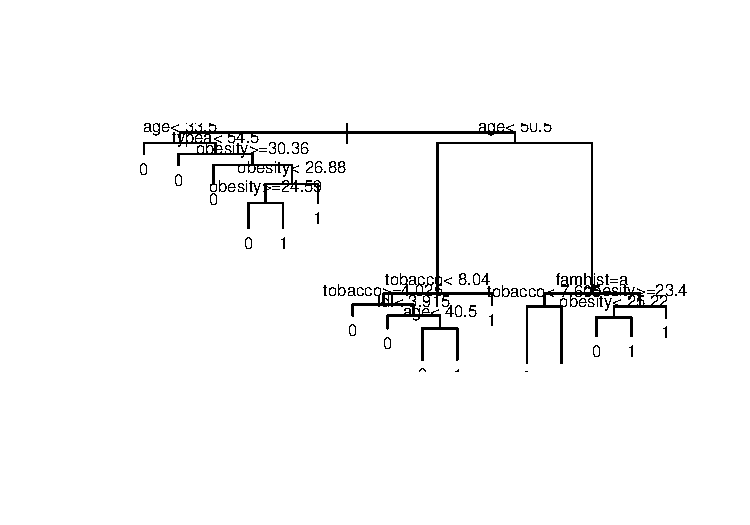
\includegraphics[width=\maxwidth]{figure/tree12} 
\begin{kframe}\begin{alltt}
\hlcomment{# optimal cp:}
tree1$cptable[\hlfunctioncall{which.min}(tree1$cptable[, \hlstring{"xerror"}]), \hlstring{"CP"}]
\end{alltt}
\begin{verbatim}
## [1] 0.01587
\end{verbatim}
\end{kframe}
\end{knitrout}

We see that we obtain the best cross validation error by fitting a tree with a complexity parameter of \texttt{0.01968504}.  Thus we prune the tree to that level. We also try prunning the tree to a smaller tree to try to compensate for over fitting.  In this case, we have to us a complexity parameter of 0.026, where, we can see form the above CP plot, that the tree size drops from 6 to 5. effective when we predict.  In the validation phase of this exercise, we can see which tree performs better on the validation set.
\begin{knitrout}
\definecolor{shadecolor}{rgb}{0.969, 0.969, 0.969}\color{fgcolor}\begin{kframe}
\begin{alltt}
\hlcomment{# selecting the optimum cp to prune the tree}
tree1.prunned1 <- \hlfunctioncall{prune}(tree1, cp = tree1$cptable[\hlfunctioncall{which.min}(tree1$cptable[, 
    \hlstring{"xerror"}]), \hlstring{"CP"}])
\hlfunctioncall{plot}(tree1.prunned1, main = \hlstring{"\hlfunctioncall{tree1.prunned1} (CP =0.019"})
\hlfunctioncall{text}(tree1.prunned1, cex = 0.7)
\end{alltt}
\end{kframe}
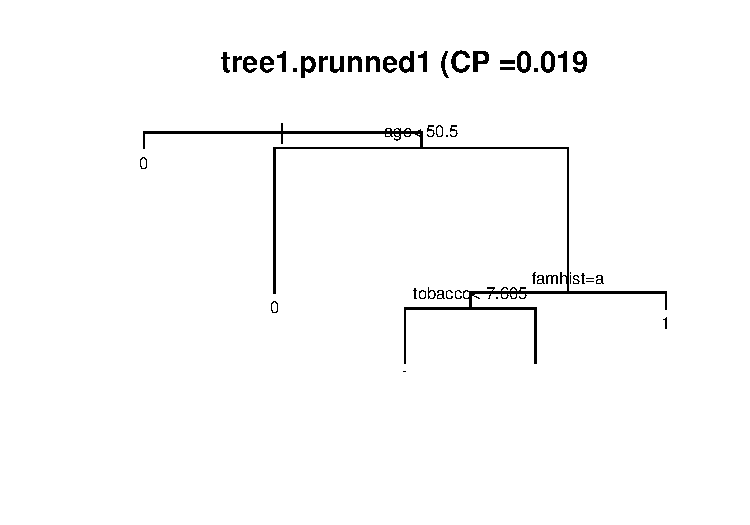
\includegraphics[width=\maxwidth]{figure/tree21} 
\begin{kframe}\begin{alltt}

tree1.prunned2 <- \hlfunctioncall{prune}(tree1, cp = 0.026)
\hlfunctioncall{plot}(tree1.prunned2, main = \hlstring{"\hlfunctioncall{tree1.prunned2} (CP=0.026"})
\hlfunctioncall{text}(tree1.prunned2, cex = 0.7)
\end{alltt}
\end{kframe}
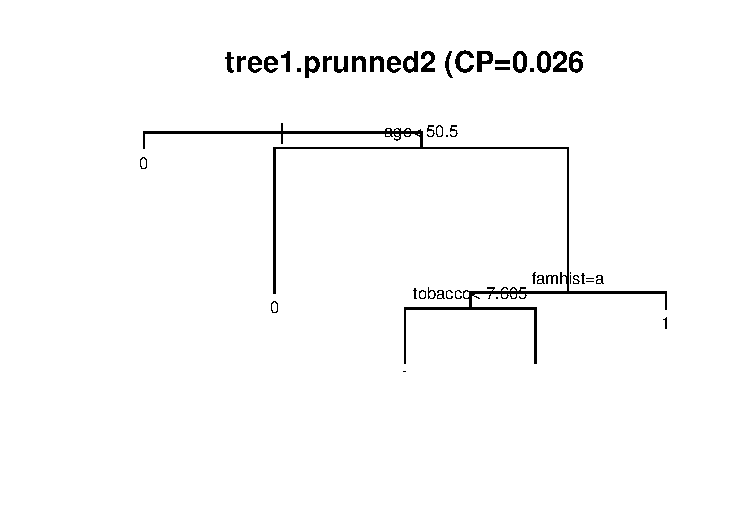
\includegraphics[width=\maxwidth]{figure/tree22} 

\end{knitrout}


\section*{Fitting a Random Forest Model}

To make this exercise slightly more interesting we can look and see how a random forest model performs on this data set, relative to a single tree.

\begin{knitrout}
\definecolor{shadecolor}{rgb}{0.969, 0.969, 0.969}\color{fgcolor}\begin{kframe}
\begin{alltt}
\hlfunctioncall{library}(randomForest)
\end{alltt}


{\ttfamily\noindent\itshape\color{messagecolor}{\#\# randomForest 4.6-7}}

{\ttfamily\noindent\itshape\color{messagecolor}{\#\# Type rfNews() to see new features/changes/bug fixes.}}\begin{alltt}
rf <- \hlfunctioncall{randomForest}(y = \hlfunctioncall{as.factor}(training.data$chd), x = training.data[, -10], 
    ntree = 100, type = \hlstring{"class"}, replace = TRUE)
\hlfunctioncall{print}(rf)
\end{alltt}
\begin{verbatim}
## 
## Call:
##  randomForest(x = training.data[, -10], y = as.factor(training.data$chd),      ntree = 100, replace = TRUE, type = "class") 
##                Type of random forest: classification
##                      Number of trees: 100
## No. of variables tried at each split: 3
## 
##         OOB estimate of  error rate: 31.22%
## Confusion matrix:
##     0  1 class.error
## 0 212 40      0.1587
## 1  78 48      0.6190
\end{verbatim}
\end{kframe}
\end{knitrout}


\section*{Predicton using Knn}

The first task in using knn is to determine the optimal k.  To find the best k, we can only use the training data and not the validation data, because in the latter scenario, we would be introducing leakage to the model fitting.  As a result, we must subest the training data in order to evaluate the effectiveness of certain k values.  The code below test gets the average of the misclassification error for 100 different test samples of size 50 withheld from the training data for each value of k from 1 to 200.

\begin{knitrout}
\definecolor{shadecolor}{rgb}{0.969, 0.969, 0.969}\color{fgcolor}\begin{kframe}
\begin{alltt}
\hlfunctioncall{library}(class)
training.data2 <- training.data
validation.data2 <- validation.data
\hlcomment{# We transform this factor variable to a numberic variable so that KNN}
\hlcomment{# works with the dataframe}
training.data2$famhist <- \hlfunctioncall{as.numeric}(\hlfunctioncall{as.factor}(training.data$famhist))
validation.data2$famhist <- \hlfunctioncall{as.numeric}(\hlfunctioncall{as.factor}(validation.data$famhist))

err <- NULL
k <- NULL
\hlfunctioncall{for} (i in 1:200) \{
    err.temp <- NULL
    \hlfunctioncall{for} (j in 1:100) \{
        kfitting.cases <- \hlfunctioncall{sample}(1:\hlfunctioncall{dim}(training.data2)[1], 45, replace = F)  \hlcomment{# randomly select 42 records to hold out}
        kvalidation.data <- training.data2[kfitting.cases, ]
        ktraining.data <- training.data2[-kfitting.cases, ]
        knn.response <- \hlfunctioncall{knn}(train = ktraining.data[, -10], test = kvalidation.data[, 
            -10], cl = ktraining.data[, 10], k = i, l = 0, use.all = TRUE)
        err.temp[j] <- \hlfunctioncall{sum}(\hlfunctioncall{abs}(\hlfunctioncall{as.numeric}(\hlfunctioncall{as.character}(knn.response)) - kvalidation.data[, 
            10]))/\hlfunctioncall{dim}(kvalidation.data)[1]
\hlcomment{        # print(err.temp[j])}
    \}
\hlcomment{    # print(err.temp)}
    err[i] <- \hlfunctioncall{mean}(err.temp)
    k[i] <- i
\}
k.values <- \hlfunctioncall{as.data.frame}(\hlfunctioncall{cbind}(k, err))
\hlfunctioncall{colnames}(k.values) <- \hlfunctioncall{c}(\hlstring{"k"}, \hlstring{"err"})


y.loess <- \hlfunctioncall{loess}(y ~ x, span = 0.75, \hlfunctioncall{data.frame}(x = k, y = err))
y.predict <- \hlfunctioncall{predict}(y.loess, \hlfunctioncall{data.frame}(x = k))
\hlfunctioncall{plot}(k, err, main = \hlstring{"Finding the best value of k"}, ylab = \hlstring{"Average Error Rate"})
\hlfunctioncall{lines}(k, y.predict, col = \hlstring{"red"}, lwd = 2)
\end{alltt}
\end{kframe}
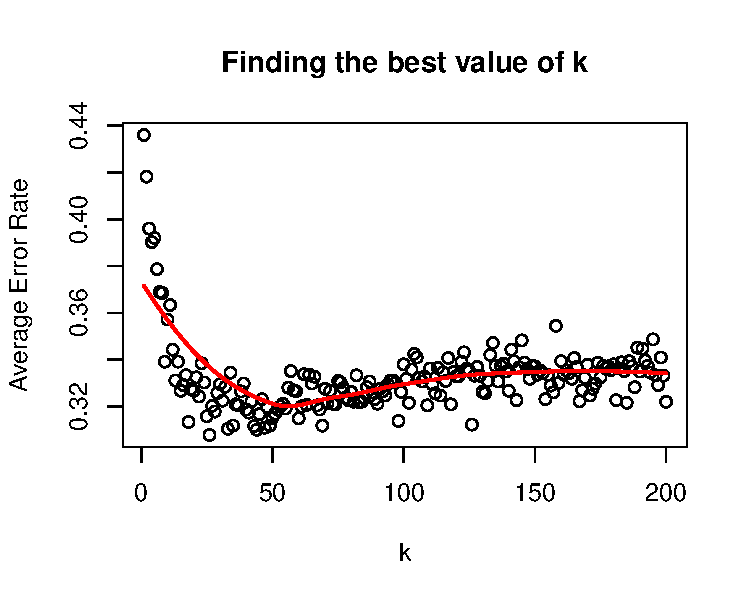
\includegraphics[width=\maxwidth]{figure/knn} 
\begin{kframe}\begin{alltt}
y.fitted <- \hlfunctioncall{unlist}(y.predict)
kmin = y.predict[\hlfunctioncall{which.min}(y.predict)]
kmin
\end{alltt}
\begin{verbatim}
##     56 
## 0.3201
\end{verbatim}
\end{kframe}
\end{knitrout}


From the above graph, we can see that a reasonable choice for k would be a value slightly larger than 50. The minimum fitted value from the loess curve (span=0.75) that we can fit to the average errors confirms that the best value for k is 56.  Thus we proceed to use that value when we apply the knn algorithm. 
\begin{knitrout}
\definecolor{shadecolor}{rgb}{0.969, 0.969, 0.969}\color{fgcolor}\begin{kframe}
\begin{alltt}
\hlcomment{# calculating the fitted values}
knn.response <- \hlfunctioncall{knn}(train = training.data2[, -10], test = validation.data2[, 
    -10], cl = training.data2[, 10], k = 56, l = 0, use.all = TRUE)
err.knn <- \hlfunctioncall{sum}(\hlfunctioncall{abs}(\hlfunctioncall{as.numeric}(\hlfunctioncall{as.character}(knn.response)) - validation.data2[, 
    10]))/\hlfunctioncall{dim}(validation.data2)[1]
err.knn
\end{alltt}
\begin{verbatim}
## [1] 0.3571
\end{verbatim}
\end{kframe}
\end{knitrout}


\section*{Prediction Using Other Models (Logistic Regression and GAM)}

We can also compare these results to logistic regression:
\begin{knitrout}
\definecolor{shadecolor}{rgb}{0.969, 0.969, 0.969}\color{fgcolor}\begin{kframe}
\begin{alltt}
logreg <- \hlfunctioncall{glm}(chd ~ ., data = training.data, family = \hlstring{"binomial"})
log.reg.pred <- \hlfunctioncall{predict.glm}(logreg, newdata = validation.data[, -10], type = \hlstring{"response"})
err.rate.log.reg <- \hlfunctioncall{sum}(\hlfunctioncall{abs}(\hlfunctioncall{round}(log.reg.pred) - validation.data[, 10]))/\hlfunctioncall{dim}(validation.data)[1]
\end{alltt}
\end{kframe}
\end{knitrout}

And we can also fit a GAM for comparison:
\begin{knitrout}
\definecolor{shadecolor}{rgb}{0.969, 0.969, 0.969}\color{fgcolor}\begin{kframe}
\begin{alltt}
\hlfunctioncall{library}(mgcv)
\end{alltt}


{\ttfamily\noindent\itshape\color{messagecolor}{\#\# This is mgcv 1.7-21. For overview type 'help("mgcv-package")'.}}\begin{alltt}
\hlfunctioncall{library}(mgcv)
\hlfunctioncall{library}(boot)
gam1 <- \hlfunctioncall{gam}(chd ~ \hlfunctioncall{s}(sbp, bs = \hlstring{"cs"}) + \hlfunctioncall{s}(tobacco, bs = \hlstring{"cs"}) + \hlfunctioncall{s}(ldl, bs = \hlstring{"cs"}) + 
    \hlfunctioncall{s}(adiposity, bs = \hlstring{"cs"}) + \hlfunctioncall{s}(typea, bs = \hlstring{"cs"}) + \hlfunctioncall{s}(obesity, bs = \hlstring{"cs"}) + 
    famhist + \hlfunctioncall{s}(alcohol, bs = \hlstring{"cs"}) + \hlfunctioncall{s}(age, bs = \hlstring{"cs"}), data = training.data, 
    family = binomial)
gam.pred <- \hlfunctioncall{predict.gam}(gam1, newdata = validation.data[, -10], type = \hlstring{"response"})
err.rate.gam <- \hlfunctioncall{sum}(\hlfunctioncall{abs}(\hlfunctioncall{round}(gam.pred) - validation.data[, 10]))/\hlfunctioncall{dim}(validation.data)[1]
\end{alltt}
\end{kframe}
\end{knitrout}




\section*{Comparing results}

First, we define a function that caclculates misclassification error for our model of interests:
\begin{knitrout}
\definecolor{shadecolor}{rgb}{0.969, 0.969, 0.969}\color{fgcolor}\begin{kframe}
\begin{alltt}
mis_class_err <- \hlfunctioncall{function}(model, validation.data = validation.data) \{
    \hlfunctioncall{if} (\hlfunctioncall{class}(model) == \hlstring{"randomForest"}) \{
        response <- \hlfunctioncall{round}(\hlfunctioncall{as.numeric}(\hlfunctioncall{as.character}(\hlfunctioncall{predict}(model, newdata = validation.data))))
        misclasserr <- \hlfunctioncall{sum}(\hlfunctioncall{abs}(response - validation.data[, 10]))/\hlfunctioncall{dim}(validation.data)[1]
    \} else \{
        response <- \hlfunctioncall{round}(\hlfunctioncall{predict}(model, newdata = validation.data)[, 2])
        misclasserr <- \hlfunctioncall{sum}(\hlfunctioncall{abs}(response - validation.data[, 10]))/\hlfunctioncall{dim}(validation.data)[1]
    \}
    \hlfunctioncall{return}(misclasserr)
\}
\end{alltt}
\end{kframe}
\end{knitrout}


Then we we combine the the results from each model into a single data frame:
\begin{knitrout}
\definecolor{shadecolor}{rgb}{0.969, 0.969, 0.969}\color{fgcolor}\begin{kframe}
\begin{alltt}
models <- NULL
err <- NULL
\hlcomment{# tree1}
models[1] <- \hlstring{"Unprunned Tree"}
err[1] <- \hlfunctioncall{mis_class_err}(tree1, validation.data)
models[2] <- \hlstring{"Prunned \hlfunctioncall{tree} (cp=0.197)"}
err[2] <- \hlfunctioncall{mis_class_err}(tree1.prunned1, validation.data)
models[3] <- \hlstring{"Prunned \hlfunctioncall{tree} (cp=0.260)"}
err[3] <- \hlfunctioncall{mis_class_err}(tree1.prunned2, validation.data)
models[4] <- \hlstring{"Random Forest"}
err[4] <- \hlfunctioncall{mis_class_err}(rf, validation.data)
models[5] <- \hlstring{"Knn"}
err[5] <- err.knn
models[6] <- \hlstring{"Regular Logistic \hlfunctioncall{Regression} (full model)"}
err[6] <- err.rate.log.reg
models[7] <- \hlstring{"Logistic \hlfunctioncall{GAM} (CS smoothed full model)"}
err[7] <- err.rate.gam

results <- \hlfunctioncall{cbind}(models, err)
\end{alltt}
\end{kframe}
\end{knitrout}


A table of our final results shows that the knn perfomed best on the held-out data followed by the prunned tree:

% latex table generated in R 2.15.1 by xtable 1.7-0 package
% Mon Apr  8 12:54:10 2013
\begin{table}[ht]
\begin{center}
\begin{tabular}{rll}
  \hline
 & models & err \\ 
  \hline
1 & Unprunned Tree & 0.285714285714286 \\ 
  2 & Prunned tree (cp=0.197) & 0.261904761904762 \\ 
  3 & Prunned tree (cp=0.260) & 0.238095238095238 \\ 
  4 & Random Forest & 0.30952380952381 \\ 
  5 & Knn & 0.19047619047619 \\ 
  6 & Regular Logistic Regression (full model) & 0.285714285714286 \\ 
  7 & Logistic GAM (CS smoothed full model) & 0.261904761904762 \\ 
   \hline
\end{tabular}
\end{center}
\end{table}
\subsection*{Discussion:}

Looking at these results, we can see that the first tree, the unprunned tree likely overfit the training data so did not perform as well on the validationd data.  Both of prunned tree models perform well, beating the regular logistic model and tying with the GAM.  The smaller model (higher CP) ends up performing better, probably because the larger model overfit the training data, like the unprunned tree.  

The random forest model (with 100 trees) did not perform particualrly well in the trial shown here, but in another trial, it only classified one record wrong (at a rate of 0.03), which indicates one of the problems with evaluating model performance on such a small held-out subset.

I am not exactly sure why that was the case, but k nearest neighboors performs very well on this data.  

Finally, we see that the parametric logistic regression model, which has many useful properties that allow interpetation of the model, does not perform as well based only on predictive performance.

To illustrate the instability of these misclassification error rates and their dependency on the sample of the 42 records that are withheld, below, are the results for each of the models for a different 42 records:
% latex table generated in R 2.15.1 by xtable 1.7-0 package
% Mon Apr  8 13:08:05 2013
\begin{table}[ht]
\begin{center}
\begin{tabular}{rll}
  \hline
 & models & err \\ 
  \hline
1 & Unprunned Tree & 0.333333333333333 \\ 
  2 & Prunned tree (cp=0.197) & 0.261904761904762 \\ 
  3 & Prunned tree (cp=0.260) & 0.261904761904762 \\ 
  4 & Random Forest & 0.30952380952381 \\ 
  5 & Knn & 0.19047619047619 \\ 
  6 & Regular Logistic Regression (full model) & 0.261904761904762 \\ 
  7 & Logistic GAM (CS smoothed full model) & 0.404761904761905 \\ 
   \hline
\end{tabular}
\end{center}
\end{table}


\end{document}
